\documentclass{article}

\usepackage{wrapfig}
\usepackage{lmodern}
\usepackage[T1]{fontenc}
\usepackage[spanish]{babel}
\usepackage{mathtools}
\usepackage{graphicx}
\usepackage[utf8]{inputenc}
\usepackage{fancyhdr}



\title{Documentación \\\large \textbf{Gigabyte B550 Aorus Master}}
\author{Antonio Muñoz Cubero}
\date{20 de Ocutbre de 2020} 


\begin{document}

\maketitle
\pagenumbering{gobble}

\begin{figure}[h]
  \centering
  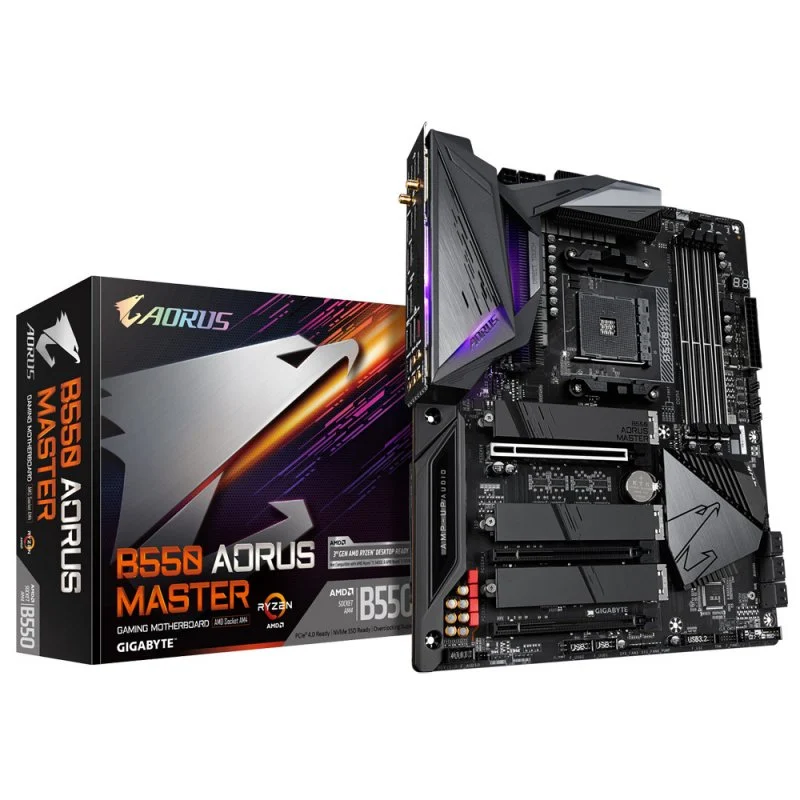
\includegraphics[scale = 0.5]{img/portada.png}
\end{figure}

\pagestyle{fancy} 

\newpage
\tableofcontents

\lhead[Documentación Placa Base]{Documentación Placa Base}
\lfoot[IES Francisco De Los Rios]{IES Francisco De Los Rios}
\pagenumbering{roman}

\section{Introducción}
Este documento contiene información sobre la placa base \textbf{B550 AORUS Master} montada por el gigante eléctrónico \textbf{Gigabyte}, esta placa introduce un nuevo chipset, que más adelante entraremos en detalle sobre el, 
el \text{B550} 
que permite montar los nuevos procesadores de \textit{AMD}, la serie 3000 y 4000.\\
Lo bueno de este chipset es que tiene un precio más ajustado al no pertenecer a la serie tope de gama de chipset y nos permite utilizar la tecnología del \textbf{PCIE 4.0}, que mas adelante desarrollaremos y entraremos en 
detalle, también 
disponemos de vaías para montar \textbf{discos duros M.2} y otras prestaciones que empezaremos a describir a continuación.

\newpage
\section{Características}

A continuación muestro una tabla con las especificanoes técnicas de la Placa Base, mas adelante iremos centrandonos en cada uno de sus aspectos.

\begin{figure}[h]
  \centering
  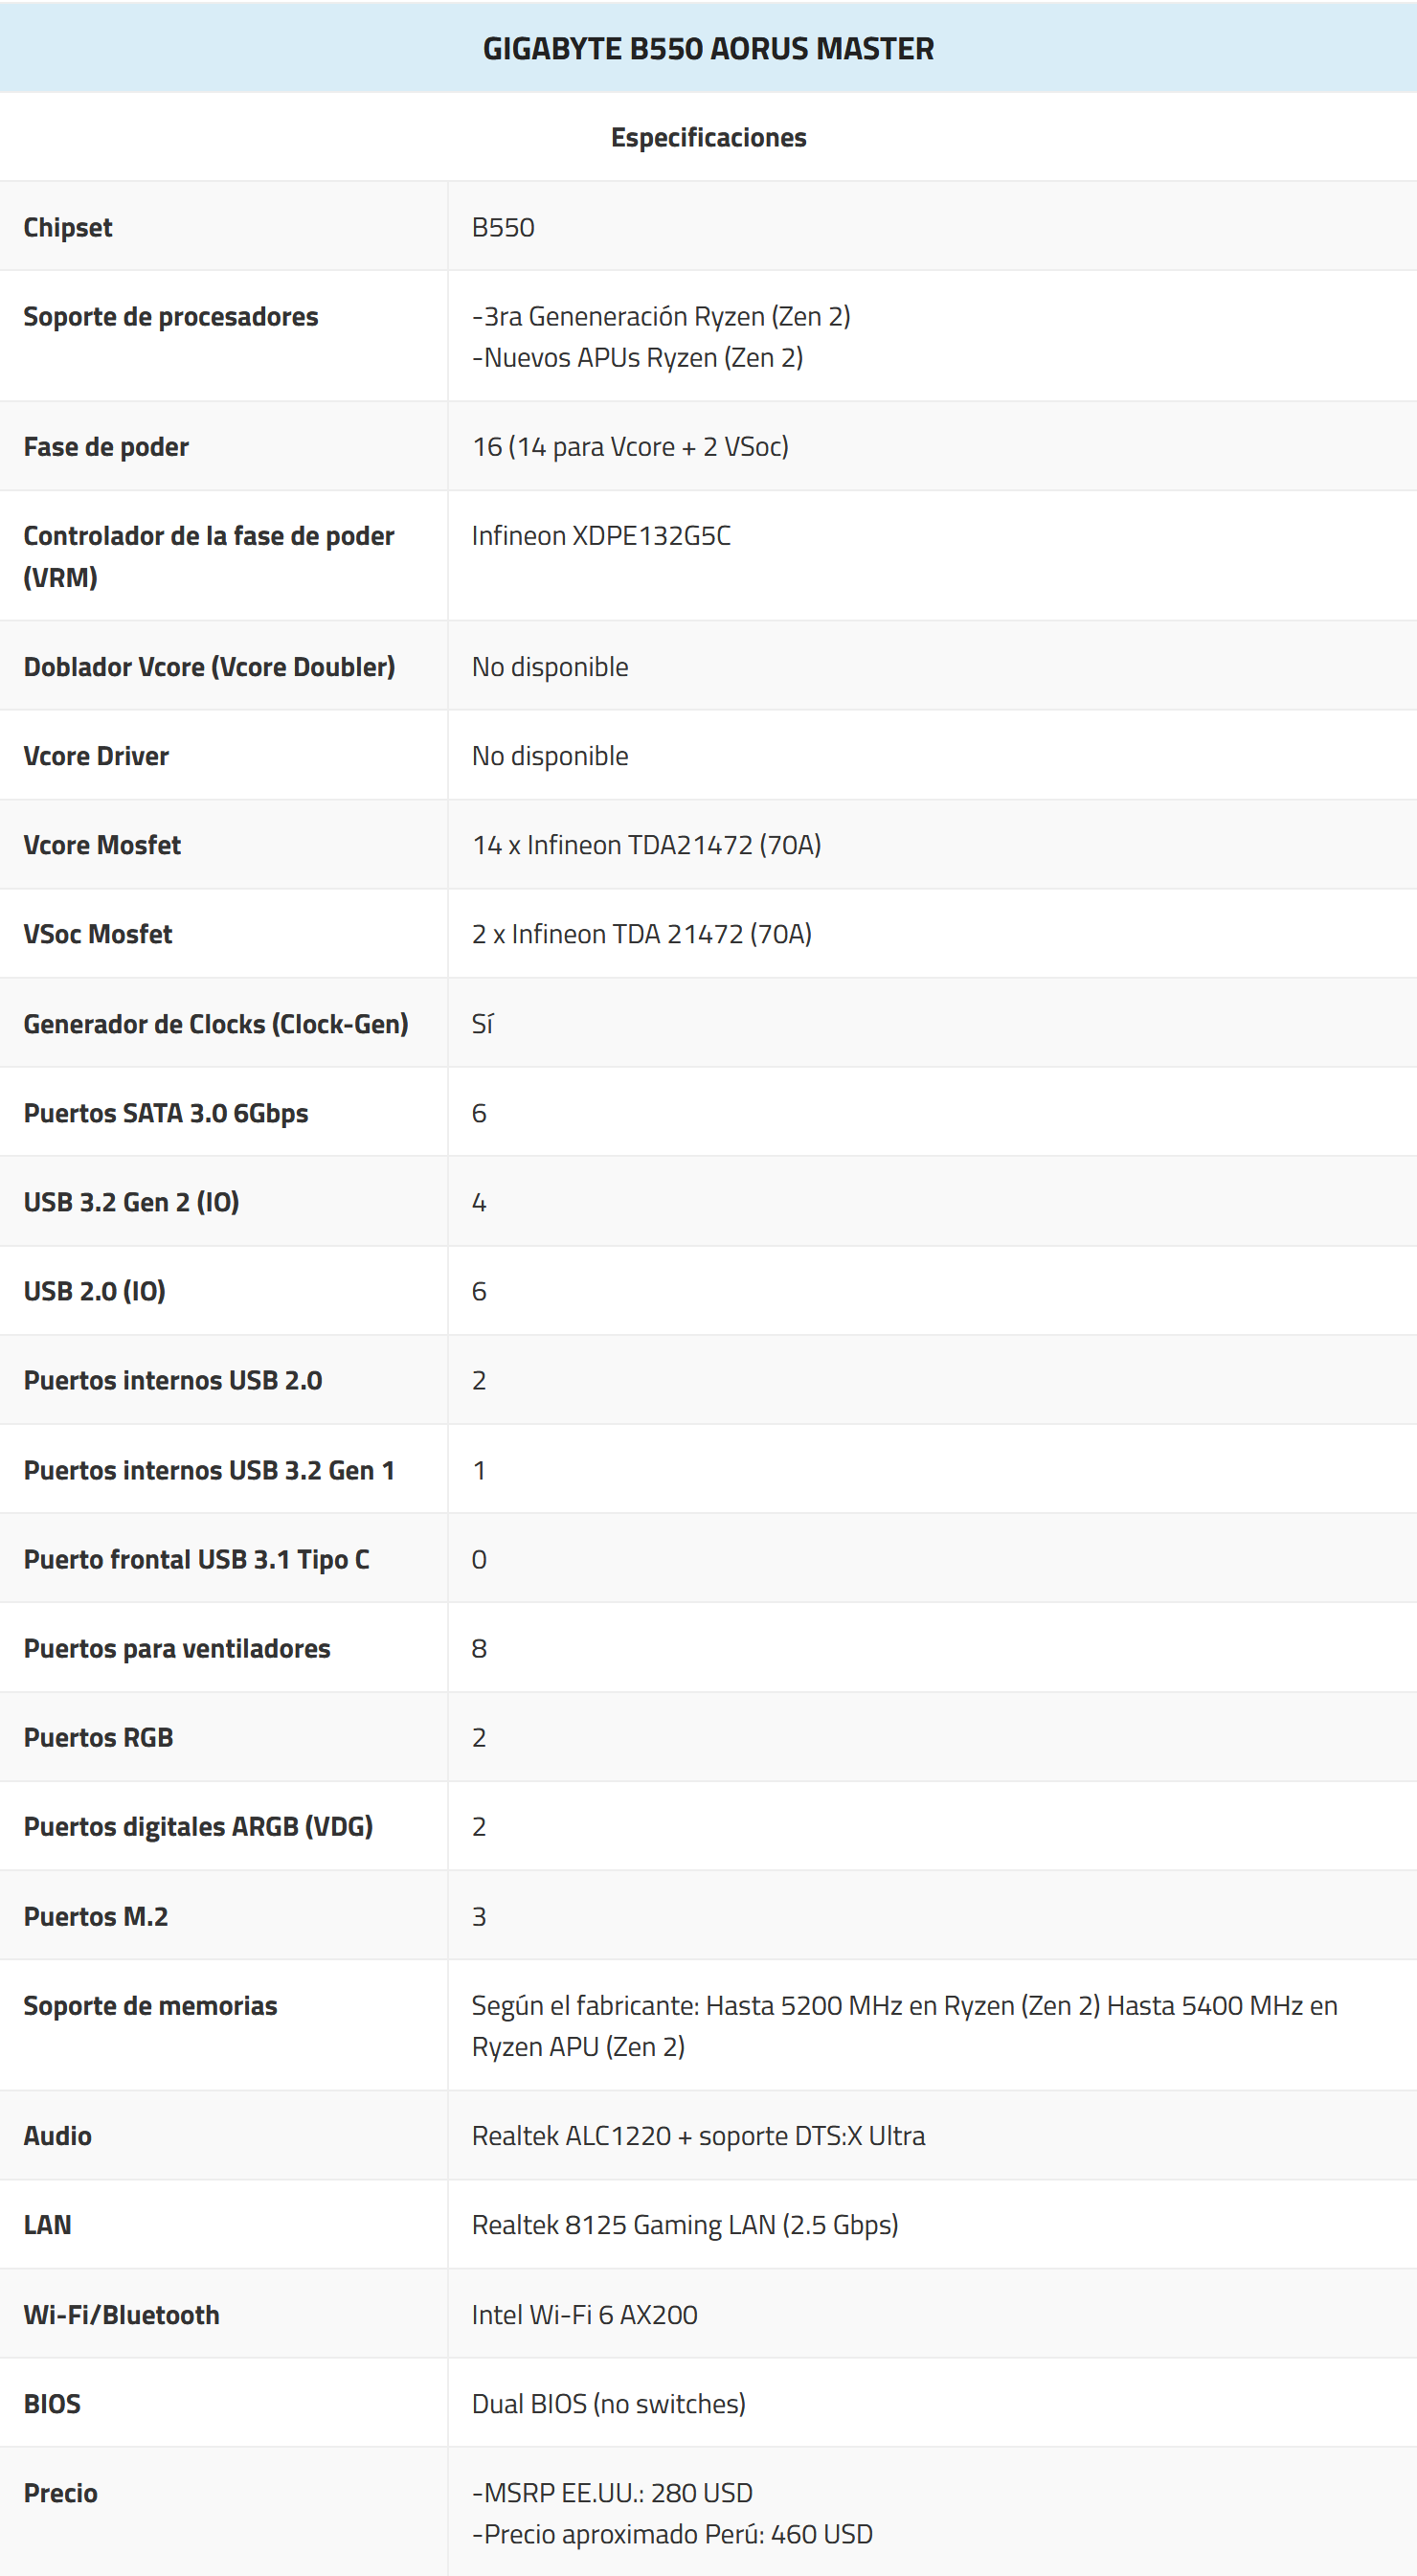
\includegraphics[scale = 0.21]{img/final_specs.png}
\end{figure}

\newpage
\subsection{Memoria RAM}

\newpage

\subsection{Conexiones Internos}

\normalsize
  {\bfseries Las conexiones internas del pc las mostramos a continuación: }% do not use \bf in LaTeX it is deprecated 20+ years ago
  \begin{itemize}
    \item Lista de Conexiones:\\
    \\
    \begin{minipage}{0.5\textwidth}
      \begin{itemize}% never number things manually!
        \item 1 x 24-pin ATX main power connector
        \item 1 x 8-pin ATX 12V power connector
        \item 1 x 4-pin ATX 12V power connector
        \item 1 x CPU fan header
        \item 1 x water cooling CPU fan header
        \item 4 x system fan headers
        \item 2 x system fan/water cooling pump headers
        \item 2 x addressable LED strip headers
        \item 2 x RGB LED strip headers
        \item 1 x CPU cooler LED strip/RGB LED strip header
        \item 3 x M.2 Socket 3 connectors
        \item 6 x SATA 6Gb/s connectors
        \item 1 x front panel header
        \item 1 x front panel audio header
        \item 1 x USB 3.2 Gen 1 header
        \item 2 x USB 2.0/1.1 headers
        \item 1 x noise detection header
        \item 1 x Trusted Platform Module
        \item 1 x Clear CMOS jumper
        \item 2 x temperature sensor headers
      \end{itemize}
    \end{minipage}
    \begin{minipage}{\textwidth}
      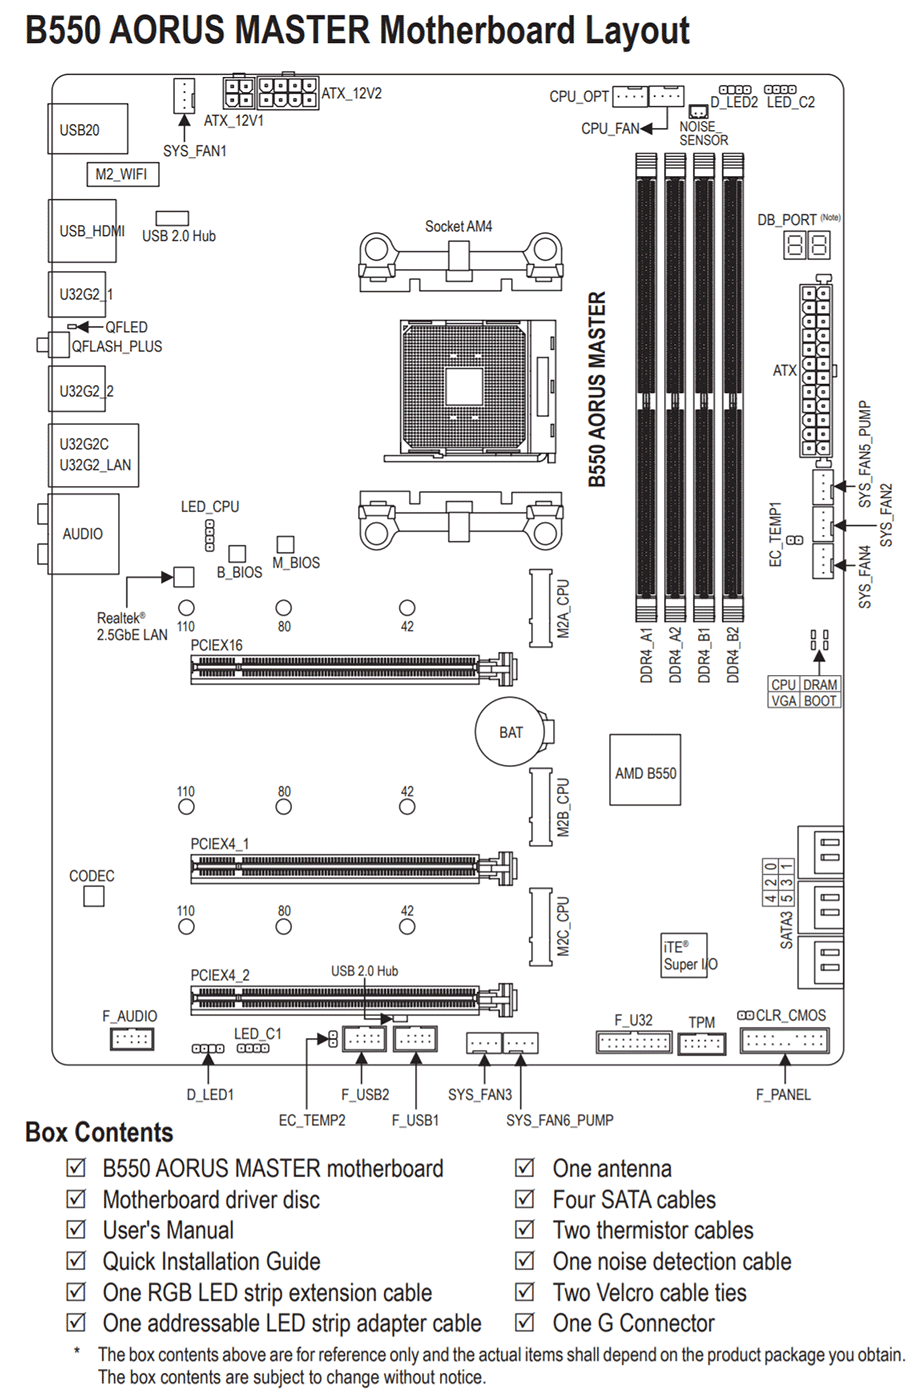
\includegraphics[scale=0.25]{img/B550AORUSMasterDiagram.png}
    \end{minipage}
  \end{itemize}

\newpage
\subsection{Conectores Externos}


\normalsize
  {\bfseries Ahora hablaremos de los \textbf{Conectores Externos} de la placa, estos son los que podemos usar para usar rapidamente las conexiones de los puertos que dispone nuestra placa, para así poder 
  externalizar las funcionalidades que nos brinda nuestro PC. }% do not use \bf in LaTeX it is deprecated 20+ years ago
  \begin{itemize}
    \item Lista de Conexiones:

    \begin{minipage}{0.5\textwidth}
      \begin{itemize}% never number things manually!
        \item x1 HDMI
        \item x6 USB 2.0/1.1
        \item X5 USB 3.2 GEN2 TYPE A
        \item X1 USB TYPE C
        \item Q-Flash Plus button
        \item X1 puerto RJ-45
        \item X5 AUDIO JACK 
        \item x1 OPTICAL S/PDIF 
      \end{itemize}
    \end{minipage}
    \begin{minipage}{\textwidth}
      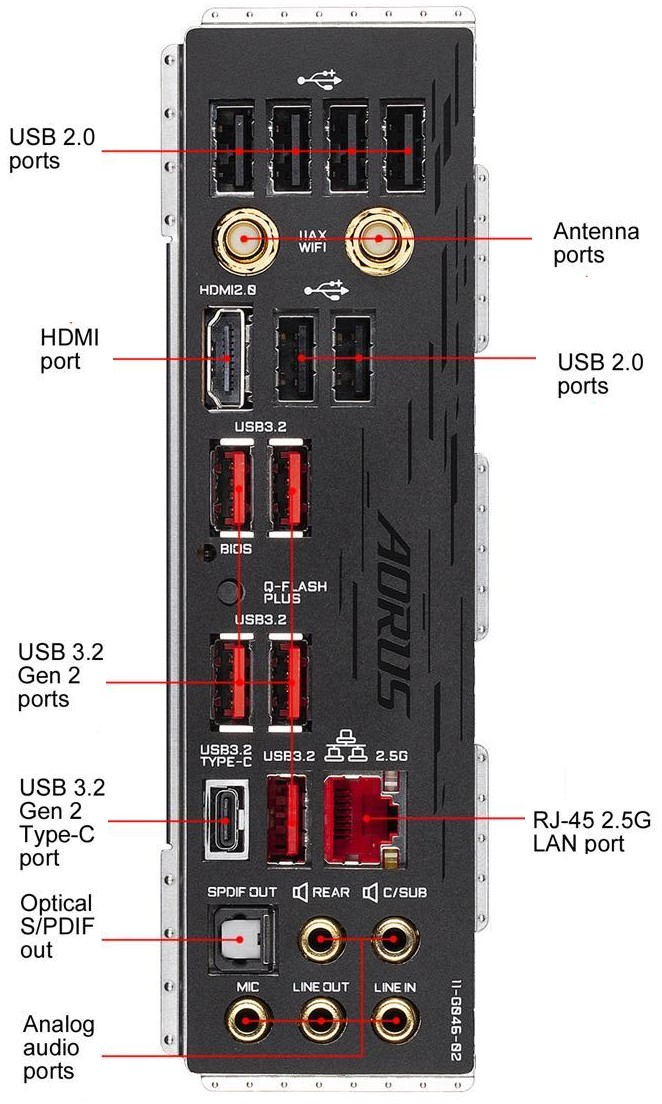
\includegraphics[scale=0.4]{img/frontal_vertical.jpg}
    \end{minipage}
  \end{itemize}


\end{document}